\chapter{Morphology}

	\section{Reduplication}

	One of \kurango 's hallmarks is its reduplicative system. It has multiple reduplicative processes.

	\subsection{Intensification}
	\label{redup_intens}
		 Semantically, this reduplicative process results in an intensification of the meaning of the morpheme. This more or less restricts where reduplication can or can not occur---it is common on intensifiable parts of speech like adjectives, and very rare on less-intensifiable parts of speech like verbs. The reduplicative template varies based on how many syllables\footnote{Syllable being one vowel and its onset, or one grapheme in the \emph{kuraito} orthography.} are in the stem.

		\subsubsection{One and two-syllable stems}
			One and two-syllable stems are copied and reduplicated entirely\footnote{Forms in these tables ignore phonological rules and represent underlying forms.}.
				\begin{table}[H]
				\centering
					\begin{tabular}{ll}
					Original Form & Reduplicated Form \\ \hline\hline
					ga -ti -xu si & ga -titi -xu si \\
					`I like someone.' & `I love someone.' \\ \hline
					ga -\N a -ka si & ga -\N a -kaka si \\
					`I am unhappy.' & `I am miserable.' \\ \hline
					\glot a\R i {-g\OO\OO} {\R\OO} & \glot a\R i {-g\OO\OO} {\R\OO\R\OO} \\
					`Please leave.' & `Go away!' \\ \hline
					ni- \glot a\N a -mi si \R i? & ni- \glot a\N a -mi si \R i\R i? \\
					`What is your name?' & `I really need to know your name.' \\
					\hline\hline 
					\end{tabular}
				\caption{One-syllable stem reduplication}
				\end{table}

				\begin{table}[H]
				\centering
					\begin{tabular}{ll}
					Original Form & Reduplicated Form \\ \hline\hline
					gaku & gakugaku \\
					`good' & `very good' \\ \hline
					ga\N a & ga\N aga\N a \\
					`bad' & `very bad' \\ \hline
					\glot a\F a & \glot a\F a\glot a\F a \\
					`Yes.' & `Of course!' \\ \hline
					\glot i\glot i & \glot i\glot i\glot i\glot i \\
					`No.' & `Absolutely not!' \\ \hline
					ka\R i -su & ka\R ika\R i -su \\
					`sleepy' & `exhausted' \\ 
					\hline\hline 
					\end{tabular}
				\caption{Two-syllable stem reduplication}
				\end{table}

		\subsubsection{Three-syllable stems and up}
		Stems that are three syllables or over undergo opposite-edge reduplication of two syllables. These two syllables are selected right-to-left and then prefixed.
				\begin{table}[H]
				\centering
					\begin{tabular}{ll}
					Original Form & Reduplicated Form \\ \hline\hline
					\glot inaka\R a -su & ka\R a\glot inaka\R a -su \\
					`boring' & `extremely boring' \\
					\hline\hline
					\end{tabular}
				\caption{Three-syllable and up stem reduplication}
				\end{table}

	\subsection{Pluralization}
		Pluralization is cause by opposite-edge reduplication. One syllable from the beginning of the word is suffixed to denote a plural entity. 
			\begin{table}[H]
			\centering
				\begin{tabular}{ll}
				Original Form & Reduplicated Form \\ \hline\hline
				\glot\OO\glot ati & \glot\OO\glot ati\glot\OO \\
				`dog' & `dogs' \\ \hline
				mi\R\OO & mi\R\OO mi \\
				`cat' & `cats' \\ \hline
				\F aa\B u & \F aa\B u\F a \\
				`home' & `homes' \\ \hline
				\end{tabular}
			\caption{Pluralization}
			\end{table}
		Monosyllabic words are pluralized using the suffix \emph{-ti} instead. This suffix probably arose from confusion regarding plural person-markers and plural pronouns both being \emph{nana, nini} and \emph{nunu}.


		\section{Valence-increasing morphology}
		\subsection{Applicatives}
			Applicatives in {\kurango} are marked using a suffix on the introduced argument, -\textipa{P}uti.
			\begin{example}
			\label{ex:nonapplicative}
				Nimotivagaana. \textipa{[nimOtiBaga:na]}
				\gll ni- {\0-} m\OO ti -\B a -ga\textipa{:} -na -\0
				2- {\erg-} die -{\caus} -{\fut} -1 -\abs
				\glt `You are going to kill me.'
				\glend
			\end{example}

			\begin{example}
			\label{ex:applicative}
				Nimotivagaana soodongu'uti. \textipa{[nigu naku mOtiBaga: sO:dONuPuti]}
				\gll ni- {\0-} m\OO ti -\B a -ga\textipa{:} -na -\0 {s\OO\textipa{:}d\OO} -\N u -\textipa{P}uti
				1- {\erg}- kill -{\caus} -{\fut} -1 -{\abs} sword {-\gen} -{\D{appl}}
				\glt `You are going to kill me with a sword.' (lit: `You made me die with a sword.')
				\glend
			\end{example}

		\subsection{Causatives}
			Causatives in {\kurango} are marked using the verbal suffix -\B a.

			\begin{example}
			\label{ex:non_causative}
				Nakumotigaa. \textipa{[nakumOtiga:]}
				\gll na- ku- m\OO ti -ga\textipa{:}
				{\D{1}}- {\D{nom}}- die -{\D{fut}}
				\glt `I am going to die.'
				\glend
			\end{example}

			\begin{example}
			\label{ex:causative}
				Namotivagaana. \textipa{[namOtiBaga:na]}
				\gll na- {\0-} m\OO ti -\B a -ga\textipa{:} -na -\0
				{\D{1}} {\D{erg}}- die -{\D{caus}} -{\D{fut}} -1 -\abs
				\glt `I am going to kill myself.' (lit: `I am going to make myself die.')
				\glend
			\end{example}

		If an agentive argument is not introduced with the causative suffix -\B a, the utterance is still grammatical, but it has a passivized 
		%what should i call this??
		 connotation to it.

		 	\begin{example}
		 	\label{ex:noncausative}
		 		Nakumotivagaa. \textipa{[nakumOtiBaga:]}
		 		\gll na- ku- m\OO ti -\B a -ga\textipa{:}
		 		1- {\nom-} die {-\caus} {-\fut}
		 		\glt `I am going to be killed' (lit: I am going to be made dead) %Is this future perfect or just future? wtf
		 		\glend
		 	\end{example} % Regloss this.
	\section{Valence-decreasing morphology} % Regloss this.
	\section{Direction-encoding morphology} % Regloss this.
	\section{Evidentiality-encoding morphology}

	%kixada = evidential adverb
		%-ngo sound, language
		%-riiti sight
		% -numungu smell
		% vafawa taste
		% tuusi touch
			% ngatuusi pain (neg touch)
				% Compared to gangapoka, which is like the perceived pain, ngatuusi has a more physiological meaning
		% miiti'a sense (holistic)
			% miiti'aa sensation

	% kura think
	% rhana know
	% -kaja real
	% -nga irreal


\subsection{Discussion of knowledge}
	Knowledge is a very important concept for {\kurango} speakers, and the topic has more depth than the English language provides.

	\emph{\G a} serves as the root noun for ``general knowledge,'' but there are many semantically-related words that refer to different types of knowledge. These lexicalized words for different types of knowledge reflects what types of knowledge {\kurango} speakers believe to be important.
		\begin{enumerate}
			\item \emph{\G a\N aka\M a} is knowledge that is false or otherwise irrelevant to the current discourse.
			\item \emph{\G amuzu} is introspective knowledge, correlating somewhat to a ``sense of self.''
			\item \emph{\G as\OO t\OO\R ii} refers to social knowledge.
			\item \emph{\G apapi'a} refers to fact-based knowledge. It does not have to be applicable in any pragmatic context.
			\item \emph{\G ana\G aa} refers to knowledge in general, sort of like ``world smarts.'' It is regarded as a high compliment and the most difficult type of knowledge to obtain.
		\end{enumerate}

% talk about how you know something
% different types of knowledge shoehorned in here too!!!!!
	% \section{Case assignment}
	In \kurango , case assignment is based on word order. Arguments to the get ergative case, and arguments to the right of the verb get absolutive case.

	\begin{example}
	\label{ex:case_wordorder_1}
		Ni'inakarana. [\textipa{niPinakaRana}]
		\gll ni- inakara -na
		2- bore -1
		\glt `You bore me.'
		\glend
	\end{example}

	\begin{example}
	\label{ex:case_wordorder_2}
		Na'inakarani. [\textipa{naPinakaRani}]
		\gll na- inakara -ni
		1- bore -2
		\glt `I bore you.'
		\glend
	\end{example}

	This ordering principle also allows us to categorize {\kurango} as a Fluid-S language, as arguments of intransitive verbs (S) pattern either with subjects of transitive verbs (S\textsubscript{A}) or objects of transitive verbs (S\textsubscript{O}) based on their position relative to the verb. Determining the way in which S patterns has to do with the semantics of the utterance: S\textsubscript{A} (marked with {\D{erg}}) has no entailment about the volition of the Agent in the action being performed, while S\textsubscript{O} (marked with {\D{abs}}) entails that the agent was volitional in the action being performed.

	\begin{example}
	\label{ex:case_erg}
		Nakari. [naka\R i]
		\gll na- kari
		1- sleep
		\glt `I sleep.' (by my own volition.)
		\glend
	\end{example}

	\begin{example}
	\label{ex:case_abs}
		Karina. [ka\R ina]
		\gll kari -na
		sleep -1
		\glt `I sleep.' (no entailment about my volition.)
		\glend
	\end{example}

	%further analysis here % I think this is OK.
		% Case assignment moved to Syntax on 12/28/15

	\section{Emotion expression}
	One of the main goals of {\kurango} was to create a language in which expression of emotional states and cognitive processes was more flexible than English. For the most part, this was a goal inspired by Anna Wierzbicka's calls for use of a natural semantic metalanguage when discussing emotion, as languages tend to differ greatly in their emotion terminology. What {\kurango} brings is a hopefully language-neutral system based on permutable morphemes.

	This design goal is reflected in an Ithkuilian way through the use of an unnatural system of suffixal morphology in that it requires speakers to really think about what exactly they want to say. However, many common emotions have lexicalized compounds to serve as everyday adjectives.

	\subsection{The emotion marker \emph{ga}} % Is ga really an adjective?
		\emph{ga} is an adjective which indicates a state of emotional being. By itself, it glosses to ``emotional'', but \emph{gaa} glosses to ``emotion.as.an.abstract.concept'' through a productive vowel lengthening rule. \emph{ga} has its own system of suffixation that allows many changes to its meaning.

			\subsubsection{Morphosyntax of \emph{ga} constructions}
				The adjective \emph{ga} has five slots upon which morphology can affix.

					\begin{table}[H]
					\centering
					\label{ga_morphosyntax}
						\begin{tabular}{cccccc}
						Root & Slot 1 & Slot 2 & Slot 3 & Slot 4 & Slot 5 \\ \hline\hline
						ga & -NEG & -PRIM/-NEUT & -EMO & -TARG & -DUR \\ \hline
						\end{tabular}
						\caption{Morphosyntax of \emph{ga}}
					\end{table}

				\begin{itemize}
					\item ``NEG'' negates all following morphology.
					\item ``PRIM/NEUT'' are two derivational modifiers for the following emotion: PRIM makes an emotion ``primal,'' while NEUT makes an emotion ``neutered.''
					\item ``EMO'' is a category for indicating explicit emotional states.
					\item ``TARG'' indicates the target of the emotion.
					\item ``DUR'' indicates the duration of the previous emotion.
				\end{itemize}

				When expressing a specific emotion (that is, not the concept of ``emotion'' in general), only EMO is mandatory. The other three slots can be omitted without affecting grammaticality, but may be included for distinguishing between more precise differences between emotions.

	\subsection{NEG, PRIM, and NEUT: derivational suffixes}
		\subsubsection{NEG}
			The NEG slot can only be occupied by one suffix, \emph{-\N a}. \emph{-\N a} negates the emotional construction that follows it.

			\begin{figure}[H] % Interlineraization examples go here.
			\label{interlin_emo_neg}

				\begin{example}
				\label{ex:interlin_emo_neg_1}
					Ganga si. [\stress ga.\N a.si]
					\gll ga -\N a si
					emotional -{\negative} \cop
					\glt `Things are not going well.'
					\glend
				\end{example}

				\begin{example}
				\label{ex:interlin_emo_neg_2}
					Gangatixupa si. [ga.\stress\N a.ti.xu.pa.si]
					\gll ga -\N a -ti -xu -pa si
					emotional -{\negative} -\D{emo:affection} -\D{targ:anim} -\D{dur:short} \cop
					\glt `I am angry at someone.'
					\glend
				\end{example}

			\caption{Examples of \emph{ganga} constructions}
			\end{figure}

		\subsubsection{PRIM}
			The PRIM suffix, -\emph{p\OO}, makes an emotion ``primal.'' This is important for making distinctions between emotions like love and lust, happiness and pleasure, anger and rage, etc.

			\begin{figure}[H] % Interlineraization examples go here.
			\label{interlin_emo_prim}

				\begin{example}
				\label{ex:interlin_emo_prim_1}
					Gapowa si. [ga.\stress p\OO.\W a.si]
					\gll ga -{p\OO} -\W a si
					emotional -\D{prim} -\D{emo:confidence} \cop
					\glt `I'm feeling courageous.'
					\glend
				\end{example}

				\begin{example}
				\label{ex:interlin_emo_prim_2}
					Gapotitifu si. [ga.\stress p\OO.ti.ti.fu si]
					\gll ga -{p\OO} -titi -\F u si
					emotional -\D{prim} -\D{emo:strong.affection} -\D{targ:null} \cop
					\glt `I'm horny.'
					\glend
				\end{example}

			\caption{Examples of \emph{gapo} constructions}
			\end{figure}

		\subsubsection{NEUT}
			The NEUT suffix, -\emph{n\OO\glot i}, makes an emotion neutered. This can either reflect a decrease in intensity, or a lack of any intensity in the cases of apathy, ambivalence, etc. Pragmatically, -\emph{n\OO\glot i} is combined with anger to denote passive-aggressiveness.

			\begin{figure}[H] % Interlineraization examples go here.
			\label{interlin_emo_neut}

				\begin{example}
				\label{ex:interlin_emo_neut_1}
					Gano'i si. [ga.\stress n\OO.ji.si]
					\gll ga -n\OO\glot i si
					emotional -\D{neut} \cop
					\glt `I'm alright, I guess.' (read in voice of whiny teenager)
					\glend
				\end{example}

				\begin{example}
				\label{ex:interlin_emo_neut_2}
					Gangano'itixu si [ga.\stress\N a.n\OO.ji.ti.xu.si]
					\gll ga -\N a -n\OO\glot i -ti -xu si
					emotional -\D{neg} -\D{neut} -\D{emo:affection} -\D{targ:anim} \cop
					\glt `It's OK. I'm fine.' (In reality, I am mad at you)
					\glend
				\end{example}

			\caption{Examples of \emph{gano'i} constructions}
			\end{figure}

	\subsection{EMO, TARG, and DUR: inflectional suffixes}
		\subsubsection{EMO}
			EMO suffixes indicate explicit emotional states. Their distinctions are based upon Paul Ekman's theories of basic emotions, but additional suffixes have been added to his proposed basic emotions:
				\begin{itemize}
					\item -\emph{ka} indicates happiness or content.
					\item -\emph{ti} indicates affection.
					\item -\emph{\W u} indicates confidence. It is commonly negated to express fear or fright (depending on duration).
					\item -\emph{t\OO} indicates excitement. It is negated to express dissapointment.
					\item -\emph{xa} indicates a sense of pride/accomplishment. It is negated to express guilt, shame, and regret, depending on duration and target. Changes in duration can mean immediate or longstanding satisfaction.
				\end{itemize}

				\begin{figure}[H] % Interlineraization examples go here.
				\label{interlin_emo}

					\begin{example}
					\label{ex:interlin_emo_1}
						Gaka si. [\stress ga.ka.si]
						\gll ga -ka si
						emotional -\D{emo:content} \cop
						\glt `Things are going well.'
						\glend
					\end{example}

					\begin{example}
					\label{ex:interlin_emo_2}
						Gangatitixu si! [ga.\stress\N a.ti.ti.xu.si]
						\gll ga -\N a -titi -xu si
						emotional -{\negative} -\D{emo:strong.affection} -\D{targ:anim} \cop
						\glt `I am repulsed (by someone)!'
						\glend
					\end{example}

					\begin{example}
					\label{ex:interlin_emo_3}
						Gangawufuda si. [ga.\stress\N a.\W u.\F u.da.si]
						\gll ga -\N a -\W u -\F u -da si
						emotional -{\negative} -\D{emo:confidence} -\D{targ:null} -\D{dur.long} \cop
						\glt `I am anxious.'
						\glend
					\end{example}

					\begin{example}
					\label{ex:interlin_emo_4}
						Gatopa si [ga.\stress t\OO.pa.si]
						\gll ga -{t\OO} -pa si
						emotional -\D{emo:excitement} -\D{dur:short} \cop
						\glt `I am surprised.'
						\glend
					\end{example}

					\begin{example}
					\label{ex:interlin_emo_5}
						Gaxamuda si [ga.\stress xa.mu.da.si]
						\gll ga -xa -mu -da si
						emotional -\D{emo:pride} -\D{targ:refl} -\D{dur:long} \cop
						\glt `I am proud of myself.'
						\glend
					\end{example}
				\caption{Examples of emotional constructions using different EMO suffixes}
				\end{figure}

					\begin{table}[H]
			\centering
			\caption{Loose English equivalents of {\kurango} emotion adjectives}
			\label{emo_permutation}
				\begin{tabular}{c|cccc}
				 & + & +\D{prim} & - & -\D{prim} \\ \hline\hline
				 \emph{-ka} & 
					 \makecell{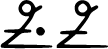
\includegraphics[scale=0.25]{././img/gaka.png}\\happiness\\contentedness} & 
					 \makecell{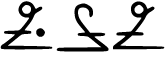
\includegraphics[scale=0.25]{././img/gapoka.png}\\pleasure\\(not nec. sexual)} & 
					 \makecell{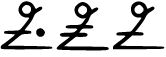
\includegraphics[scale=0.25]{././img/gangaka.png}\\unhappiness\\discontent\\sadness, anger(strong)} & 
					 \makecell{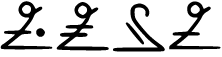
\includegraphics[scale=0.25]{././img/gangapoka.png}\\pain\\displeasure} \\
				 \emph{-ti} & 
					 \makecell{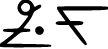
\includegraphics[scale=0.25]{././img/gati.png}\\affection\\(often romantic)} & 
					 \makecell{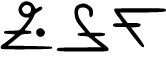
\includegraphics[scale=0.25]{././img/gapoti.png}\\lust\\wanting, craving} &
					 \makecell{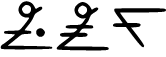
\includegraphics[scale=0.25]{././img/gangati.png}\\disdain\\detest(stronger)} &
					  \makecell{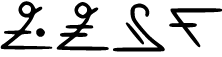
\includegraphics[scale=0.25]{././img/gangapoti.png}\\repulsion\\disgust} \\
				 \emph{-\W u} & 
					 \makecell{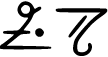
\includegraphics[scale=0.25]{././img/gawu.png}\\confidence} &
					 \makecell{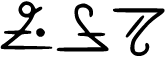
\includegraphics[scale=0.25]{././img/gapowu.png}\\courage} &
					 \makecell{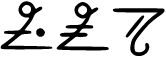
\includegraphics[scale=0.25]{././img/gangawu.png}\\doubt\\anxiety} &
					 \makecell{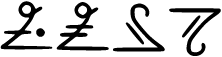
\includegraphics[scale=0.25]{././img/gangapowu.png}\\fear} \\
				 \emph{-t\OO} &
					 \makecell{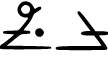
\includegraphics[scale=0.25]{././img/gato.png}\\excitement} &
					 \makecell{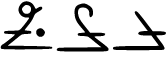
\includegraphics[scale=0.25]{././img/gapoto.png}\\arousal} &
					 \makecell{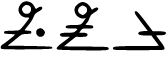
\includegraphics[scale=0.25]{././img/gangato.png}\\dissapointment} &
					 \makecell{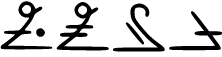
\includegraphics[scale=0.25]{././img/gangapoto.png}\\helplessness}\\
				 \emph{-xa} &
					 \makecell{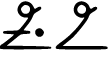
\includegraphics[scale=0.25]{././img/gaxa.png}\\pride} &
					 \makecell{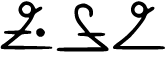
\includegraphics[scale=0.25]{././img/gapoxa.png}\\acceptance\\self of belonging} &
					 \makecell{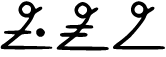
\includegraphics[scale=0.25]{././img/gangaxa.png}\\shame} &
					 \makecell{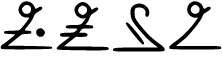
\includegraphics[scale=0.25]{././img/gangapoxa.png}\\reclusiveness\\lack of belonging} \\ \hline
				\end{tabular}
			\end{table}

		\subsubsection{TARG}
			The TARG suffixes indicate the target of the emotion. There are four possibilities for this morphosyntactic category:
				\begin{itemize}
					\item -\emph{xu} represents an animate target. This can be a person or an animal (anything with consciousness).
					\item -\emph{\F u} represents no target. It is also the inanimate suffix for a lot of constructions, and it can serve that purpose here too (eg: mad at your washing machine), but an inanimate pronoun usually follows to provide context in an ambiguous environment.
					\item -\emph{mu} is a reflexive target.
					\item -\emph{\R u} is a reciprocal target.
				\end{itemize}

			\begin{figure}[H] % Interlineraization examples go here.
			\label{interlin_emo_targ}

				\begin{example}
				\label{ex:interlin_emo_targ_1}
					Gakaxu si. [ga.\stress ka.xu.si]
					\gll ga -ka -xu si
					emotional -\D{emo:content} -\D{targ:anim} \cop
					\glt `I am content (with someone).'
					\glend
				\end{example}

				\begin{example}
				\label{ex:interlin_emo_targ_2}
					Gakafu si. [ga.\stress ka.\F u.si]
					\gll ga -ka -\F u si
					emotional -\D{emo:content} -\D{targ:null} \cop
					\glt `I am content.'
					\glend
				\end{example}

				\begin{example}
				\label{ex:interlin_emo_targ_3}
					Gakamu si. [ga.\stress ka.mu.si]
					\gll ga -ka -mu si
					emotional -\D{emo:content} -\D{targ:refl} \cop
					\glt `I am content (with myself).'
					\glend
				\end{example}

				\begin{example}
				\label{ex:interlin_emo_targ_4}
					Gakaru si. [ga.\stress ka.\R u.si]
					\gll ga -ka -\R u si
					emotional -\D{emo:content} -\D{targ:recip} \cop
					\glt `I am am in a state of mutual content with another person.' % Is there a better way to gloss this? lol...
					\glend
				\end{example}
			\caption{Examples of emotional constructions using different TARG suffixes}
			\end{figure}

		\subsubsection{DUR}
			DUR suffixes are often omitted in common conversation, and used primarily to parse apart the subtle differences between discrete emotions.
				\begin{itemize}
					\item The long durative -\emph{da} indicates that the emotion occurred for a long period of time, something like the distinction between an emotion and a mood.
					\item The short durative -\emph{pa}, on the other hand, marks the emotion as a fleeting state.
				\end{itemize}

			\begin{figure}[H] % Interlineraization examples go here.
			\label{interlin_emo_dur}

				\begin{example}
				\label{ex:interlin_emo_dur_1}
					Gatirupa si. [ga.\stress ti.\R u.pa.si]
					\gll ga -ti -\R u -pa si
					emotional -\D{emo:affection} -\D{targ:recip} -\D{dur:short} \cop
					\glt `I am in love.' (fleeting)
					\glend
				\end{example}

				\begin{example}
				\label{ex:interlin_emo_dur_2}
					Gatiruda si. [ga.\stress ti.\R u.da.si]
					\gll ga -ti -\R u -da si
					emotional -\D{emo:affection} -\D{targ:recip} -\D{dur:long} \cop
					\glt `I am in love.' (longstanding)
					\glend
				\end{example}

			\caption{Examples of emotional constructions using different DUR suffixes}
			\end{figure}

	\subsection{Reduplication}
		Like other morphological categories in {\kurango}, EMO, DUR, TARG, PRIM, NEUT, and NEG can be reduplicated in order to modify intensity. It is interesting to note that reduplicating the PRIM suffix creates the lexicalized expression akin to the word ``fuck'' in English in terms of distribution and meaning. Etymologically, this comes from expressions like (\ref{ex:interlin_emo_prim_2}), which is the most common usage of \emph{po}.



	\section{Numeracy}

	\subsection{The cardinal root \emph{\R\OO}}
		Cardinal numbers in {\kurango} are marked with the cardinal root \emph{\R\OO}. The vowel can be lengthened to form \emph{\R\OO\OO}, ``number'' as an abstract concept. However, it more commonly appears with the numeracy suffixes, discussed below.
	\subsection{Numeracy suffixes}
		\kurango 's capacity to encode any number comes from the combination of ten morphemes that represent the numbers 0-9. These morphemes have underlying forms that obey syllable structure rules for \kurango, but they are commonly discussed as though they only have consonants in their stems. This is because of an overarching vowel harmony rule based on whether or not the initial numeral suffix is odd or even (see below). 
		% couldn't get autoref to properly work here
			\begin{table}[H]
			\centering
			\caption{{\kurango} numeracy suffixes}
			\label{numeracy_table}
				\begin{tabular}{c|ccc}
					Numeral & Suffix & -a glyph & -u glyph \\ \hline\hline
					1 & -xa\R a & 
						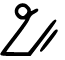
\includegraphics[scale=0.25]{././img/1A.png} &
						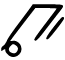
\includegraphics[scale=0.25]{././img/1U.png} \\
					2 & -duzu &
						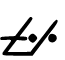
\includegraphics[scale=0.25]{././img/2A.png} &
						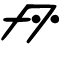
\includegraphics[scale=0.25]{././img/2U.png} \\
					3 & -ta\R a &
						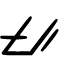
\includegraphics[scale=0.25]{././img/3A.png} &
						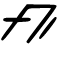
\includegraphics[scale=0.25]{././img/3U.png} \\
					4 & -kutu &
						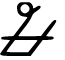
\includegraphics[scale=0.25]{././img/4A.png} &
						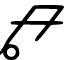
\includegraphics[scale=0.25]{././img/4U.png} \\ 
					5 & -sa\N a &
						
\includegraphics[scale=0.25]{././img/5A.png} &
						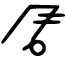
\includegraphics[scale=0.25]{././img/5U.png} \\
					6 & -zusu &
						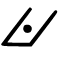
\includegraphics[scale=0.25]{././img/6A.png} &
						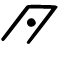
\includegraphics[scale=0.25]{././img/6U.png} \\
					7 & -sata &
						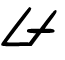
\includegraphics[scale=0.25]{././img/7A.png} &
						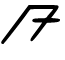
\includegraphics[scale=0.25]{././img/7U.png} \\
					8 & -\glot u\glot u &
						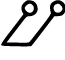
\includegraphics[scale=0.25]{././img/8A.png} &
						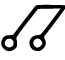
\includegraphics[scale=0.25]{././img/8U.png} \\
					9 & -na\B a &
						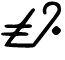
\includegraphics[scale=0.25]{././img/9A.png} &
						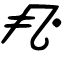
\includegraphics[scale=0.25]{././img/9U.png} \\
					0 & -zu\R u &
						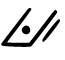
\includegraphics[scale=0.25]{././img/0A.png} &
						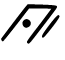
\includegraphics[scale=0.25]{././img/0U.png} \\ \hline
				\end{tabular}
			\end{table}

		So, \emph{roxara} would gloss to ``one,'' but these suffixes can also attach to nouns. An example would be \emph{o'atikutu}, or "four dogs."

		\subsubsection{Larger numbers and vowel harmony}
		\label{number_harmony}
			A language should, naturally, have a way to discuss really large numbers. In \kurango, this is as simple as attaching multiple suffixes to \emph{\R\OO}. However, there is a catch:

				\begin{figure}[H]
				\label{interlin_num_harm}
					\begin{example}
					\label{num_a_harm}	
						roxarazarasata [\R\OO.\stress xa.\R a.za.\R a.sa.ta]
						\gll {\R\OO} -xa\R a -zu\R u -sata
						\D{num} -one -zero -seven
						\glt `one hundred seven'
						\glend
					\end{example}

					\begin{example}
					\label{num_u_harm}
						*roxarazurusata [\R\OO.\stress xa.\R a.zu.\R u.sa.ta]
						\gll {\R\OO} -xa\R a -zu\R u -sata
						\D{num} -one -zero -seven
						\glt `(Intended) one hundred seven'
						\glend
					\end{example}
				\end{figure}

			As stated earlier, there is an overarching vowel harmony rule based on whether or not the initial numeral suffix is odd or even. Looking at the numeracy suffixes above, a noticeable pattern emerges, where odd numeral suffixes have /a/ as their vowels and even numeral suffixes (and zero) have /u/ as their vowels. The suffix that attaches closest to the root \emph{\R\OO} determines the vowel harmony for the rest of the numeral construction.

	\subsection{Ordinality}
		Ordinality in {\kurango} is a lot more simple than English ordinality. There are no semantic classes of objects that take different ordinal morphology (take ``tertiary'' versus ``third'')---all take the same derivational suffix \emph{-ta}. For example, \emph{o'atitakutu} would translate to ``the fourth dog'' (compare with \emph{o'atikutu} ``four dogs'' above).

		\subsubsection{Ordinality and calendar terms}
			The ordinal suffix is used on the roots ``year,'' ``day,'' ``week,'' and ``month'' to express calendar terms.

			\begin{itemize}
			\item \emph{di} is the root for ``day.'' \emph{ditaxa\R ana\B a} would translate to ``the nineteenth day,'' and \emph{dixa\R ana\B a} to ``nineteen days.''

			\item \emph{\glot u} is the root for ``week.'' \emph{\glot uta\glot u\glot uzu\R u} would translate to ``the eightieth week,'' and \emph{\glot u\glot u\glot uzu\R u} to ``eighty weeks.''

			\item \emph{m\OO} is the root for ``month.'' \emph{m\OO tata\R a} would translate to ``March (lit: the third month),'' and \emph{m\OO ta\R a} to ``three months.''

			\item \M i is the root for ``year.'' \emph{\M itaduzuzu\R uxu\R usu\N u} would translate to ``2015 (lit: the 2015th year),'' and \emph{\M iduzuzu\R uxu\R usu\N u} to ``2015 years.''
			\end{itemize}

	\subsection{Multiplicative adverbs}
		Cardinal number constructions can be derived into multiplicative adverbs ``double, triple, quadruple'' as they can in English, using an additional root that is mutually exclusive with the noun slot. This root is \emph{d\OO\R\OO}. An example would be \emph{d\OO\R\OO sata}, which translates to ``septuple.''

	\subsection{Morphosyntax}
		\begin{table}[H]
		\centering
		\label{num_morphosyntax}
			\begin{tabular}{cccc}
			Root & Slot 1 & Slot 2 & Slot 3-$\infty$ \\ \hline\hline
			\makecell{\R\OO\\d\OO\R\OO\\any noun} & \makecell{-ti\\
			%-d\OO THIS WAS IN THIS SLOT ALSO, WHAT DOES IT MEAN
			} & \makecell{Numeracy suffix\\(that determines vowel harmony)} & \makecell{Numeracy suffix\\(that undergoes vowel harmony)} \\ \hline
			\end{tabular}
			\caption{Morphosyntax of numeracy constructions}
		\end{table}

	\subsection{Other useful numeracy constructions}
		There are several other common constructions where numeracy suffixes come in handy.

		\begin{itemize}
			\item Last names: \emph{\glot a\N ataduzu} ``last name (lit: second name)''
			\item Secondary emotions: \emph{gatitixu si ga\N a\W u\F upataduzu si} ``I love someone, but I am also scared (lit: I love someone; my second emotion is fear)'' % May not be grammatically correct. Possibly missing something like ``but''
		\end{itemize}

% Dont forget: lengthening of last vowel for turning a morpheme into a noun.

% Talk about unlimited (virtually?) zero derivation

